% !TEX encoding = UTF-8 Unicode
% !TEX TS-program = XeLaTeX
\documentclass{beamer}

\usetheme{metropolis}

\usepackage[utf8]{inputenc} % Prevent wrong encoding

\usepackage{nameref} % References with names
\usepackage{caption} % Small captions
\usepackage[inline]{enumitem} % customisable lists
\usepackage{subcaption} % Subcaptions

\usepackage[french]{babel}

% Theme elements configuration
\metroset{numbering=fraction,
          subsectionpage=progressbar,
          block=fill}

\setitemize{label=\textbullet}

\title{Sokoban}
%\subtitle{The subtitle}
\date{\today}
\author{Maël Querré\\
    Alexis Mortelier\\
    Vincent De Menezes\\
    Christina Williamson}
\institute{Université de Caen Normandie}

\begin{document}

\maketitle

% Table des matières
% ===================
\begin{frame}[allowframebreaks]{Table des matières}
  \setbeamertemplate{section in toc}[sections numbered]
  \tableofcontents[sections={1-3}]
    \framebreak
  \tableofcontents[sections={4-}]
\end{frame}

% Introduction
% ============
\metroset{sectionpage=none} % Do not show the section page since there is subsection
\section{Introduction}
\metroset{sectionpage=progressbar} % Reset
\subsection{Description du projet}\label{project-desc}
\begin{frame}{\nameref{project-desc}}
  \begin{block}{Sokoban}
    Jeu de puzzle composé de cases ayant chacune un type défini.
  \end{block}
  
  \vspace{1em}
  
  \begin{block}{Types de cases}
    \begin{itemize*}[label=] % no label
      \item vide,
      \item mur,
      \item caisse,
      \item joueur,
      \item cible,
      \item caisse sur cible,
      \item joueur sur cible
    \end{itemize*}
  \end{block}
  
  \vspace{1em}
  
  
\includegraphics{images/default/0.png}\hspace{1em}
  
\includegraphics{images/default/1.png}\hspace{1em}
  
\includegraphics{images/default/2.png}\hspace{1em}
  
\includegraphics{images/default/3.png}\hspace{1em}
  
\includegraphics{images/default/4.png}\hspace{1em}
  
\includegraphics{images/default/5.png}\hspace{1em}
  
\includegraphics{images/default/6.png}
\end{frame}

\begin{frame}{Objectif du projet}
  \begin{center}
    Intelligence artificielle capable de jouer en simultané avec un joueur sur le jeu Sokoban.
    \vfill
    \begin{figure}
      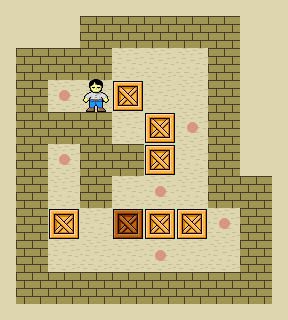
\includegraphics[height=.4\textheight]{images/sokoban_example.png}
      \caption{Un plateau de jeu de Sokoban classique}
    \end{figure}
  \end{center}
\end{frame}

\begin{frame}{Objectif du projet}
  \begin{block}{Travail demandé}
    \begin{itemize}
      \item importation de niveaux
      \item interface graphique
      \item résolution automatique de niveau (intelligence artificielle)
    \end{itemize}
  \end{block}
\end{frame}

\metroset{sectionpage=none} % Do not show the section page since there is subsection
\section{Organisation}
\metroset{sectionpage=progressbar} % Reset
\subsection{Répartition du travail}
\begin{frame}{Répartition du travail}
  \begin{block}{Répartition en 3 parties}
    \begin{itemize}
      \item Conception et représentation du jeu
      \item Interface graphique
      \item Intelligence artificielle
    \end{itemize}
  \end{block}
\end{frame}

\subsection{Déroulement du travail}
\begin{frame}
  \frametitle{Journal de groupe du déroulement du travail pendant les séances}
  \begin{itemize}
    \item DE MENEZES Vincent :\\
      \begin{itemize}
        \item Les deux premières séances :\\
          Etablissement du plan\\
          Conception du jeu (plateau et case)
        \item 3ième à 5ième séances :\\
          Optimisation de certaines méthodes\\
          Correction de certains bugs\\
          Vérification du jeu par test
        \item 6ième séances :\\
          Mise au point du projet\\
          Adaptation de l'interface graphique au projet du groupe\\
        \item 7ième séances :\\
          Correction de bug causé par l'implémentation des autres parties du projet
      \end{itemize}
  \end{itemize}
\end{frame}
\begin{frame}
  \frametitle{Journal de groupe du déroulement du travail pendant les séances}
    \begin{itemize}
      \item DE MENEZES Vincent (suite):
      \begin{itemize}
        \item Les dernière séances :\\
          Recherche sur le fonctionnement des résolutions de plateau du Sokoban\\
          Recherche sur l'algorithme A*\\
          Conception de l'intelligence artificielle\\
          Rédaction rapport et soutenance\\
          Intégration de l'IA dans le projet comun\\
      \end{itemize}
      \item MORTELIER Alexis
      \begin{itemize}
        \item Seance 1 :\\
          Architecture du projet UML et répartition des taches
        \item Seance 2 à 4 :\\
          Conception du jeu (plateau et chargement du niveau)
      \end{itemize}
    \end{itemize}
\end{frame}
\begin{frame}
  \frametitle{Journal de groupe du déroulement du travail pendant les séances}
    \begin{itemize}
      \item MORTELIER Alexis (suite):
      \begin{itemize}
        \item Seance 5 à 7:\\
          Test des méthodes, correction de bug et d'erreurs, optimisation des methodes
        \item Seance 8 :\\
          impplémentation du MVC Pattern
        \item Seance 9 et 10:\\
          implémentation de l'editeur de level completement indépendant avec interface graphique respectant le MVC Pattern  
      \end{itemize}
    \end{itemize}
\end{frame}

% Architecture du projet
% ======================
\metroset{sectionpage=none} % Do not show the section page since there are subsections
\section{Architecture}
\metroset{sectionpage=progressbar} % Reset
\subsection{Structure principale}
\begin{frame}{Structure principale}
  Arborescence inspirée de \emph{Apache Maven} :
  \begin{itemize}
    \item \texttt{src/main/java} : sources principales
    \item \texttt{src/main/resources} : ressources principales
    \item \texttt{src/test/java} : sources de tests
    \item \texttt{src/test/resources} : ressources de tests
  \end{itemize}
\end{frame}

\subsection{Structure des packages}
\begin{frame}{Structure des packages}
  Classes regroupées par fonctionnalité
  \begin{figure}
    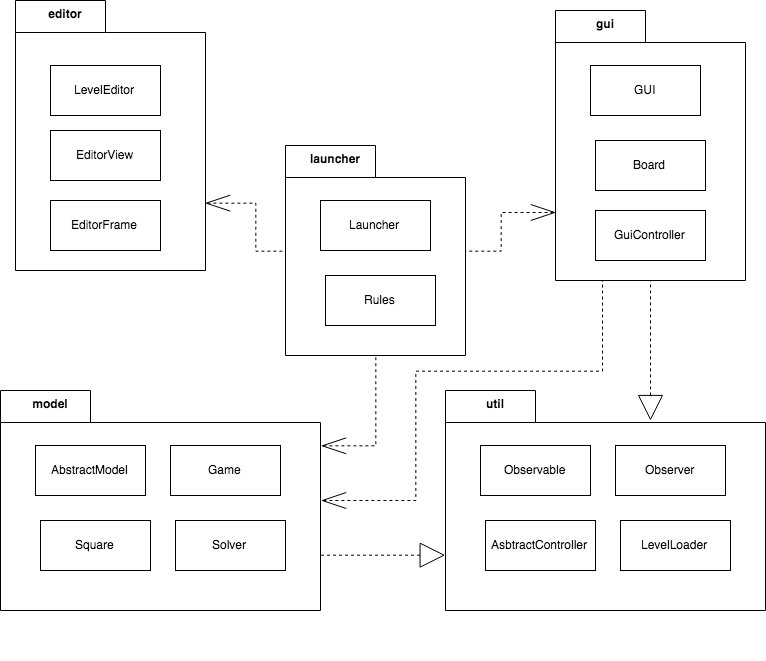
\includegraphics[width=.7\textwidth]{images/packages.png}
    \vspace{-1em}
    \caption{Diagramme de packages}
  \end{figure}
\end{frame}

% Éléments techniques
% ===================
\section{Éléments techniques}
\begin{frame}{Termes techniques}
  \vfill
  \begin{block}{Jeu bloqué}
    Plateau possédant une caisse sur une case gelée.
  \end{block}
  \vfill
  \begin{block}{Case gelée}
    Case dont les axes horizontal et vertical sont bloqués
  \end{block}
  \vfill
  \begin{block}{Axe bloqué}
    Il existe un mur ou une case bloquée sur les cases voisines de l'axe
  \end{block}
\end{frame}

\begin{frame}{Termes techniques}
  \vfill
  \begin{block}{Case bloquée}
    Vérifie qu'elle possède un axe bloqué 
  \end{block}
  \vfill
  \begin{alertblock}{Observation}
    Une case bloquée possédant 2 axes bloqués devient une case gelée
  \end{alertblock}
\end{frame}


% Fonctionnalités implémentées
% ============================
\metroset{sectionpage=none} % Do not show the section page since there are subsections
\section{Fonctionnalités implémentées}
\metroset{sectionpage=progressbar} % Reset
\subsection{Expérimentations et usages}\label{exp-and-usages}

\begin{frame}{\nameref{exp-and-usages}}
  \begin{block}{Conception du jeu}
    Présentation de la conception du jeu
  \end{block}
\end{frame}

\begin{frame}{\nameref{exp-and-usages}}
  \begin{block}{Intelligence artificielle}
    Présentation de l'intelligence artificielle
  \end{block}
  \begin{center}
    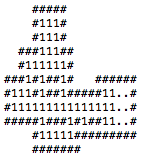
\includegraphics[width=.3\textwidth]{images/check.png}
    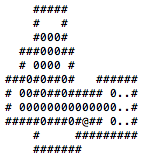
\includegraphics[width=.3\textwidth]{images/deadlock.png}
    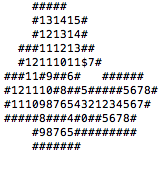
\includegraphics[width=.3\textwidth]{images/radar.png}
  \end{center}
\end{frame}

\begin{frame}{\nameref{exp-and-usages}}
  \begin{block}{Éditeur de niveau}
    Présentation de l'éditeur de niveau
  \end{block}
\end{frame}

\subsection{Interface graphique}
\begin{frame}{Éléments du jeu}
\vfill
\begin{figure}
\subcaptionbox*{vide}{
\includegraphics{images/custom/0.png}}\hspace{.5em}
\subcaptionbox*{mur}{
\includegraphics{images/custom/1.png}}\hspace{.5em}
\subcaptionbox*{caisse}{
\includegraphics{images/custom/2.png}}\hspace{.5em}
\subcaptionbox*{joueur}{
\includegraphics{images/custom/3.png}}\hspace{.5em}
\subcaptionbox*{cible}{
\includegraphics{images/custom/4.png}}\hspace{.5em}
\subcaptionbox*{caisse sur cible}{
\includegraphics{images/custom/5.png}}\hspace{.5em}
\subcaptionbox*{joueur sur cible}{
\includegraphics{images/custom/6.png}}
\end{figure}
\end{frame}

\begin{frame}{Lanceur de jeu}
  \begin{figure}
    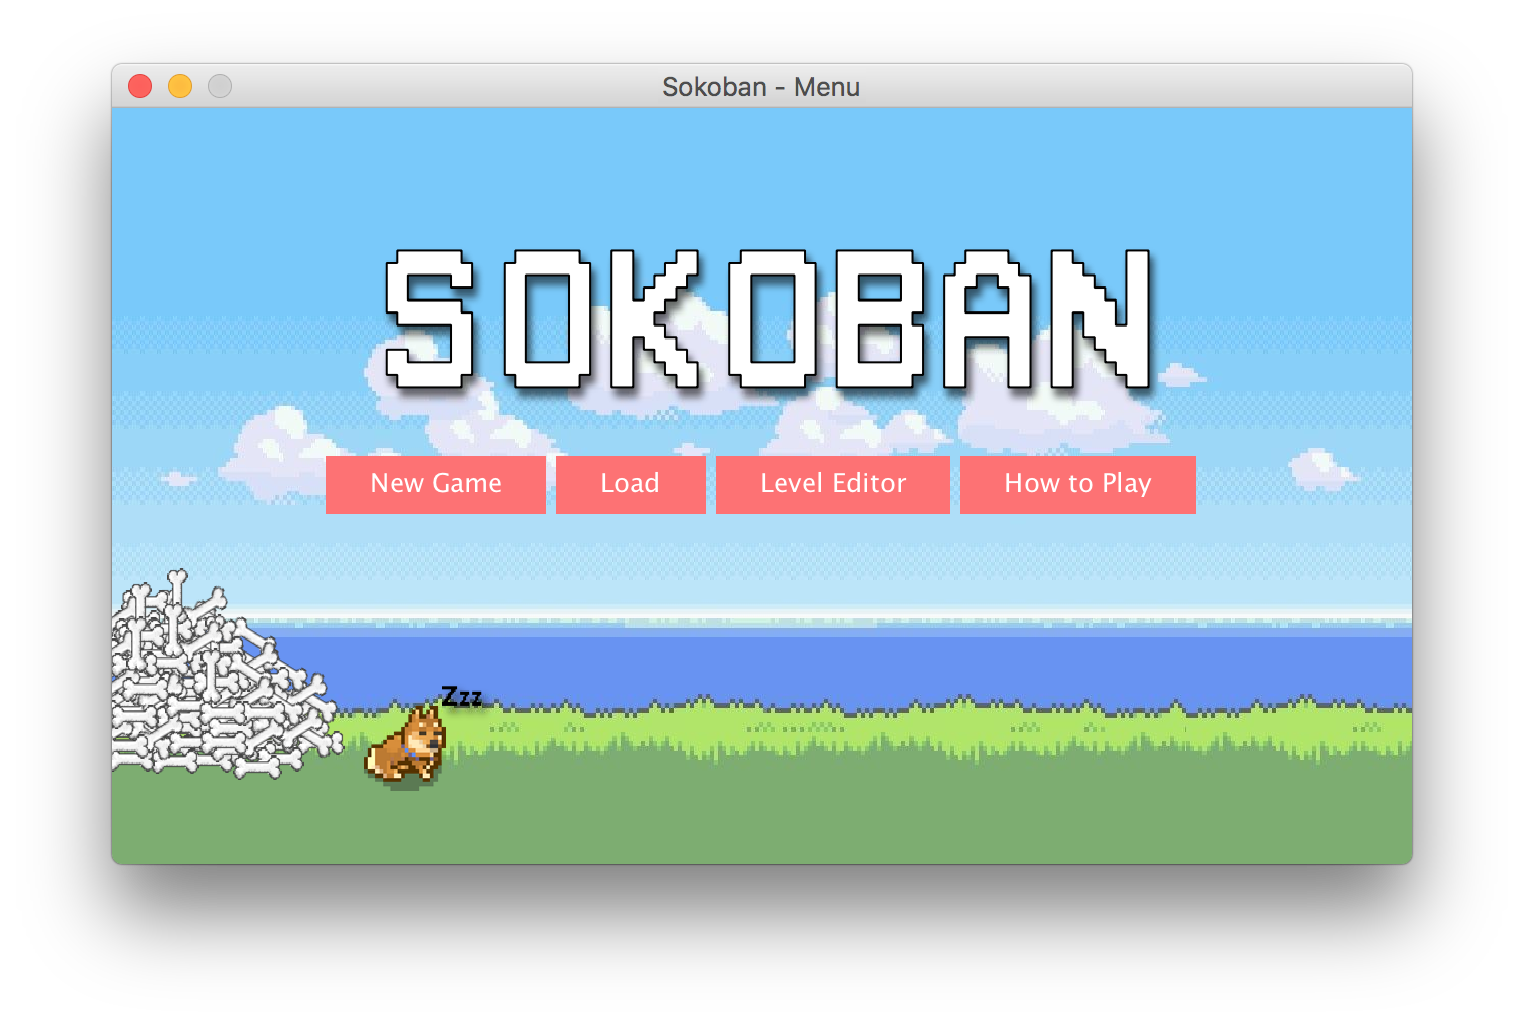
\includegraphics[width=.9\textwidth]{images/launcher.png}
    \vspace{-2em}
    \caption{Le lanceur du jeu}
  \end{figure}
\end{frame}

\begin{frame}{Comment jouer}
  \begin{figure}
    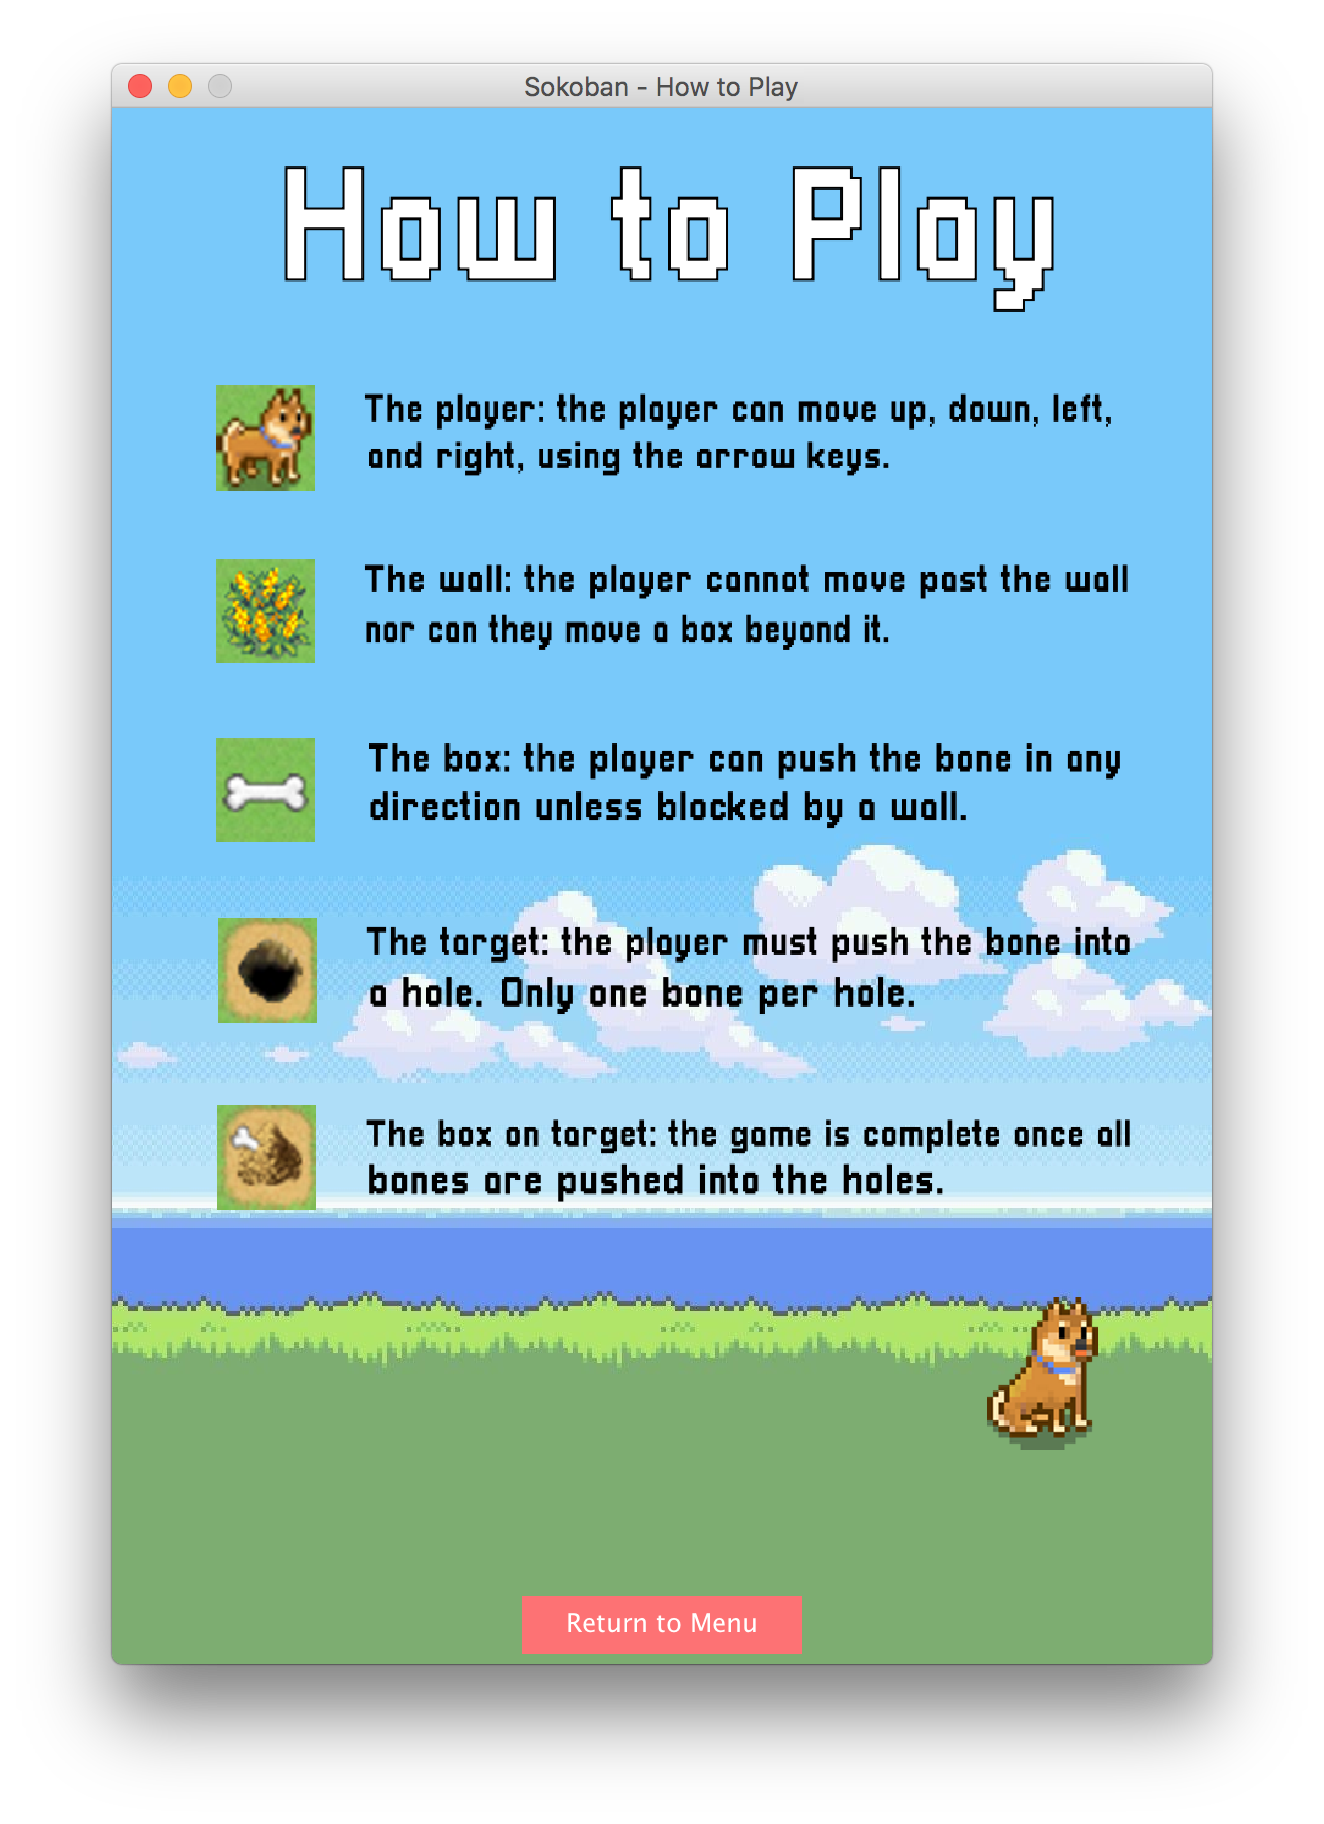
\includegraphics[height=.8\textheight]{images/rules.png}
    \vspace{-1em}
    \caption{La fenêtre "comment jouer"}
  \end{figure}
\end{frame}

\begin{frame}{Le jeu}
  \begin{figure}
    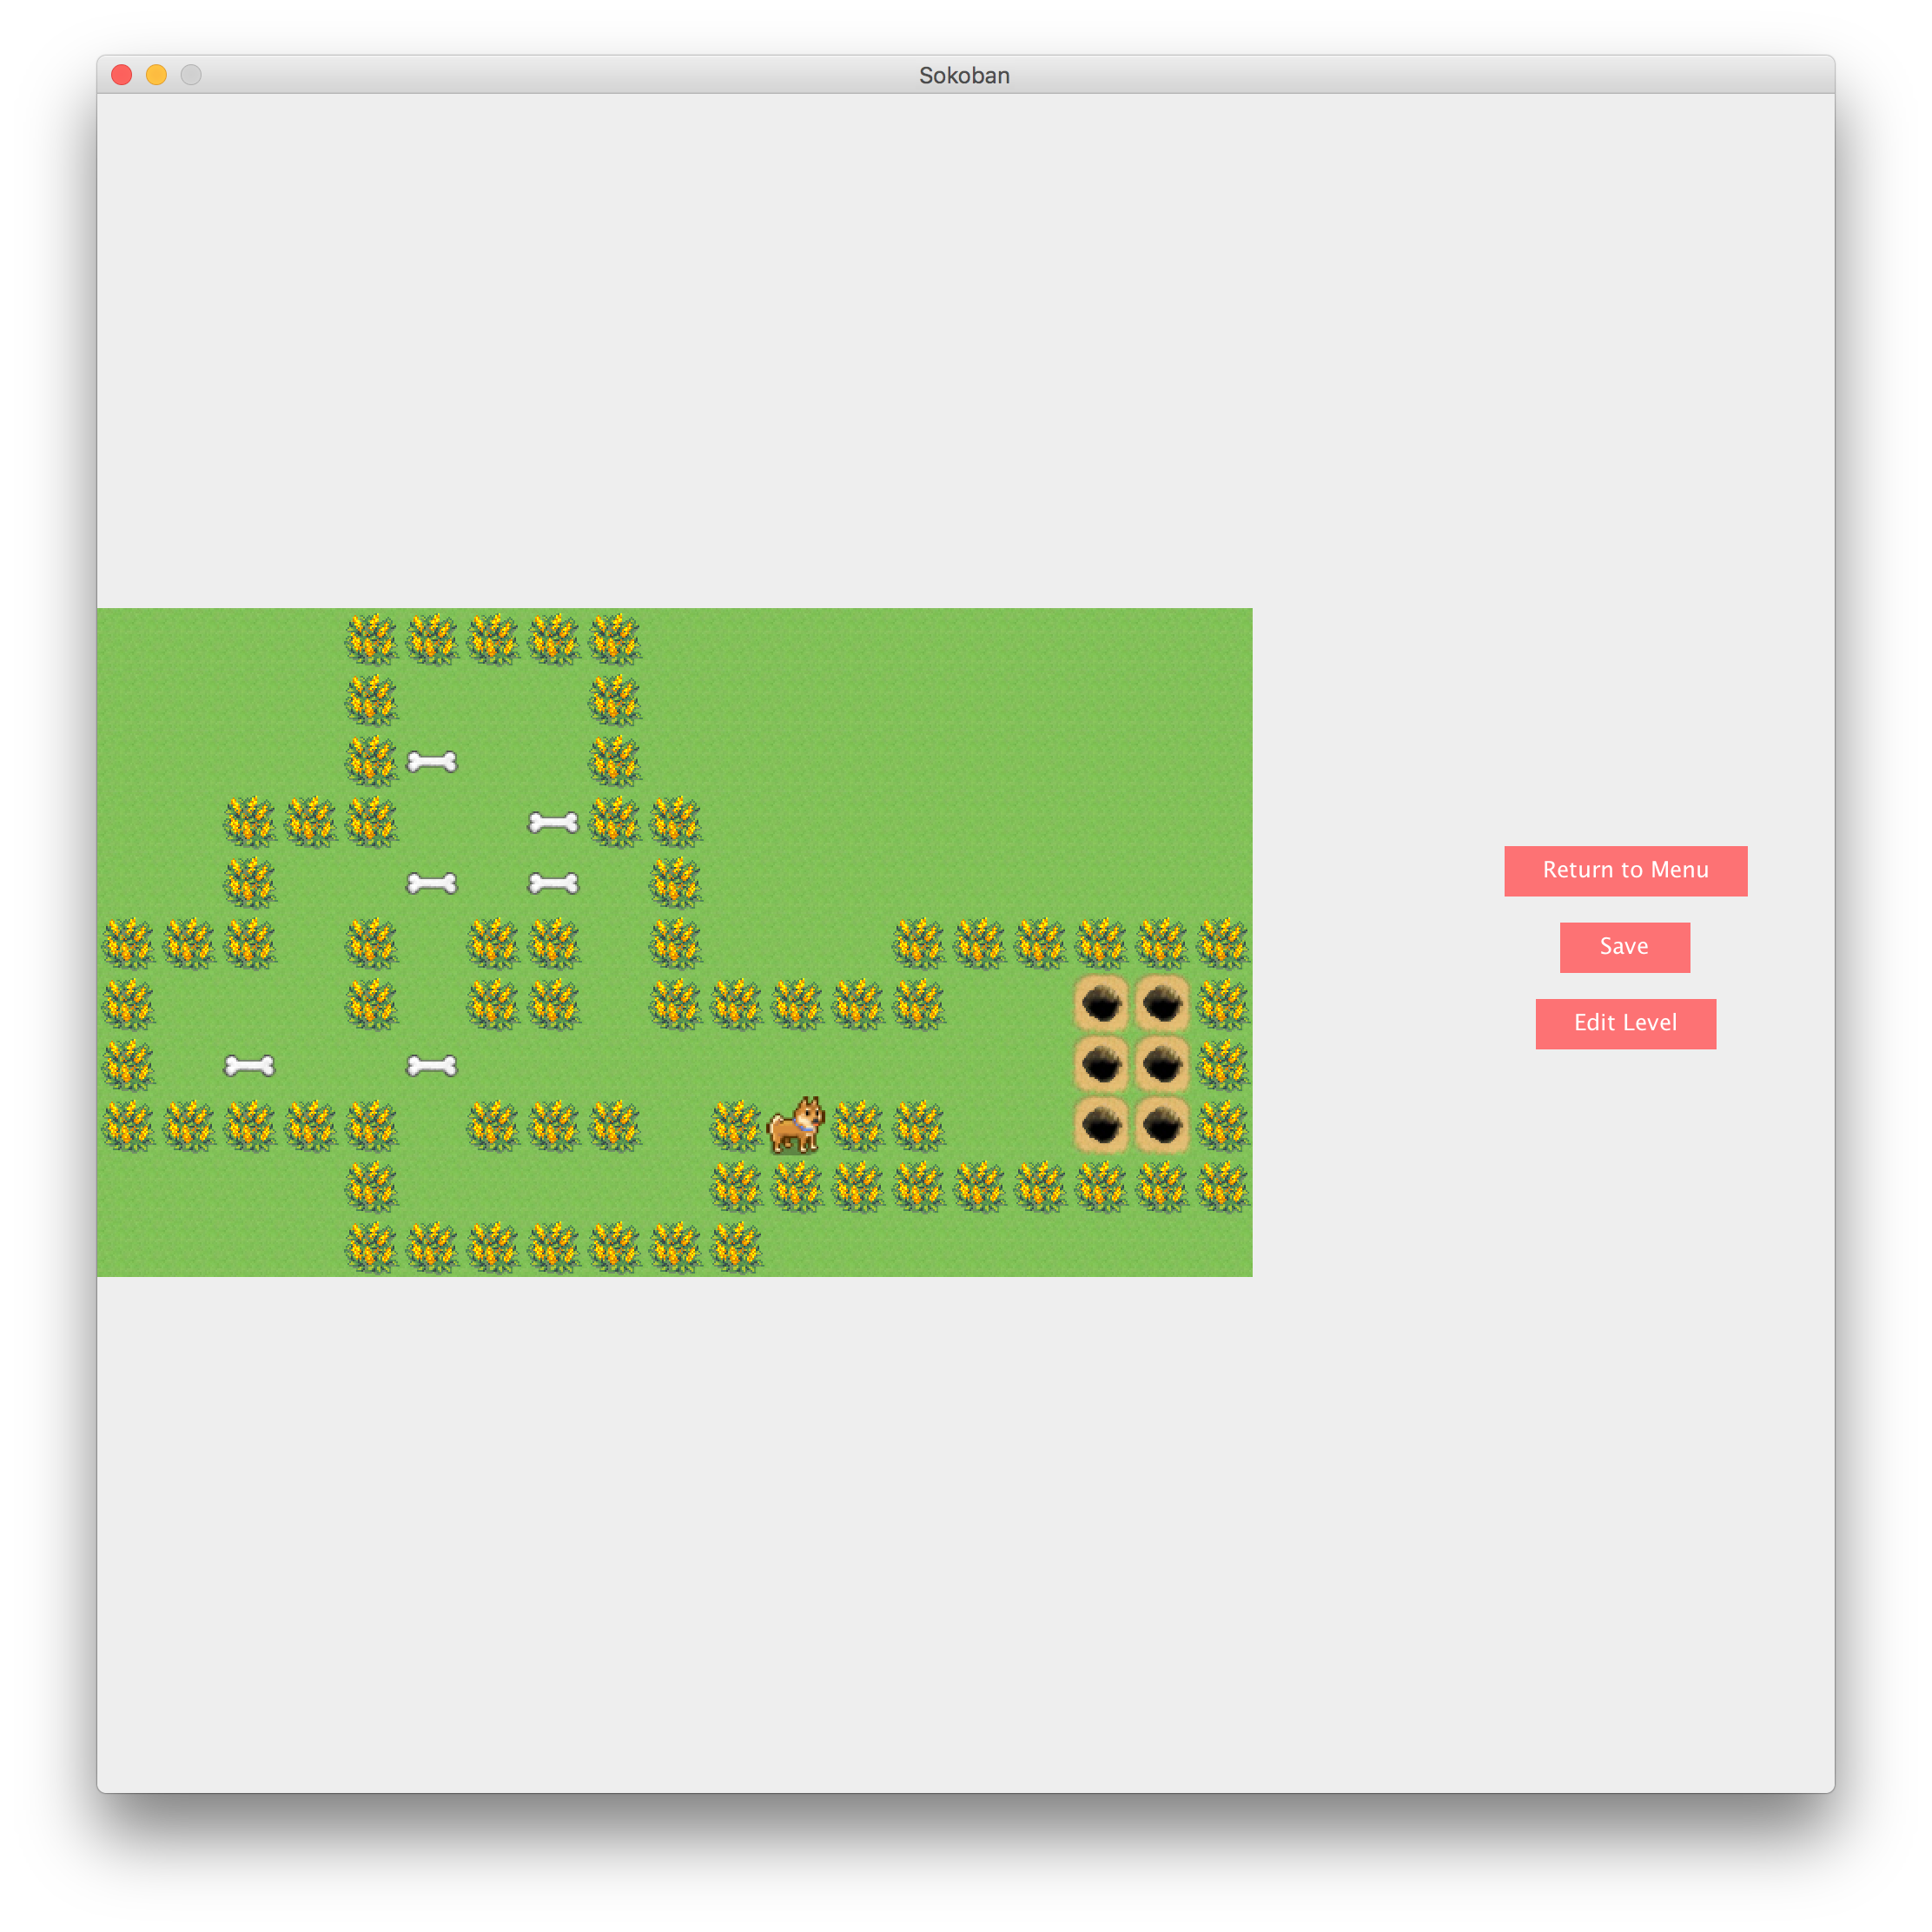
\includegraphics[width=.7\textwidth]{images/game.png}
    \vspace{-1em}
    \caption{Un jeu de Sokoban}
  \end{figure}
\end{frame}

\begin{frame}{Éditeur de niveau}
  \begin{figure}
    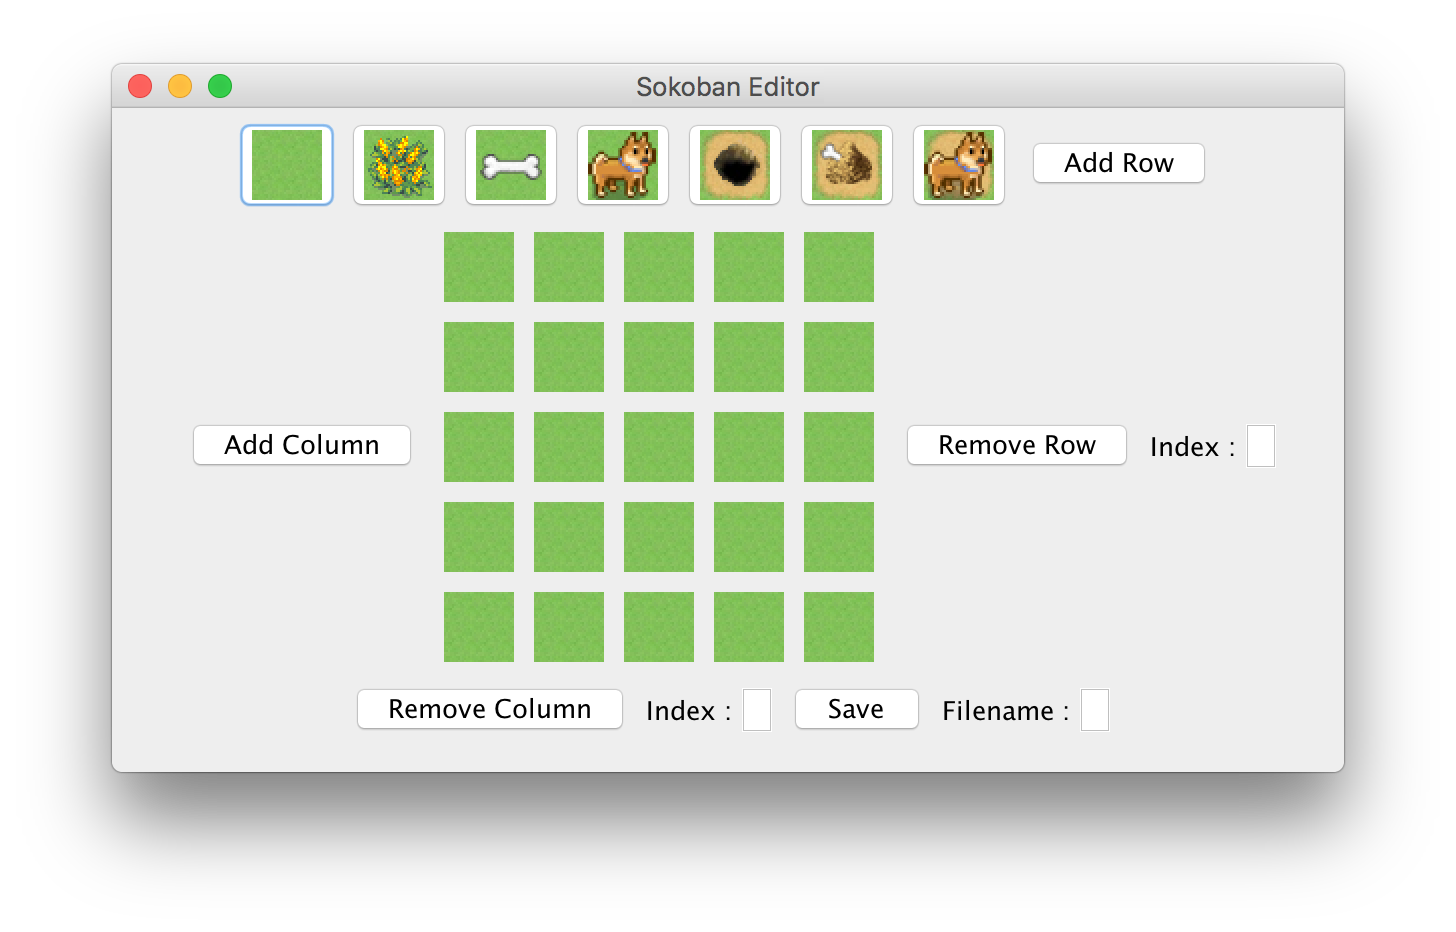
\includegraphics[width=\textwidth]{images/editor.png}
    \vspace{-2em}
    \caption{L'éditeur de niveau}
  \end{figure}
\end{frame}

% Conclusion
% ==========
\metroset{sectionpage=progressbar} % Ensure that the Conclusion section page is displayed
\section{Conclusion}
\begin{frame}{Propositions d'améliorations}
  \begin{block}{Une représentation du jeu différente}
    Utilisation d'ensembles pour regrouper les cases du plateau
  \end{block}
  \vfill{}
  \begin{block}{Mode coopération}
    Deux joueurs sur un même plateau
  \end{block}
\end{frame}

\begin{frame}[standout]
  Merci de votre attention
\end{frame}

\end{document}
